\chapter{SMART MAC Analysis}
\label{cap:apendiceA}

The purpose of this appendix is discussing how the SMART Memory Access Control (SMART MAC) was implemented. Also, some tests will be showed and commented. Below, at code box \ref{code:core}, is possible to see the core code of the of the module. The module header and parameters initializations are not showed because they do not influence in the module behaviour. 

Although the small size of the module, it has a reasonable complexity.  The microcontroller clock synchronize all actions taken by the module.  This mechanism is important because sometimes, during a fetch, decode or execution of an instruction in the microcontroller, the value of some pins, like the instruction pointer or the memory address, can become a random number. This strange behaviour happens because when a 16 bits bus changes its value, the bits are not changed together. This time variation is very small, but if the module does not use a sycronize mechanism, an incorrect reset signal can be produced. 
\newline

\begin{lstlisting}[caption={Core code of the SMART MAC},label={code:core}]
module  smart_mac (
	// OUTPUTs
	output                  in_safe_area,       // On on safe area
	output                  reset,              // High to reset device
	output           [15:0] mem_dout,           // Memory data output
	
	// INPUTs
	input [SIZE_MEM_ADDR:0] mem_addr,           // Memory adress
	input                   mclk,               // Memory clock
	input            [15:0] mem_din,            // Memory data input
	input            [15:0] ins_addr,           // Instruction pointer adress
	input                   disable_debug       // Disable protection on HIGH
);

// PARAMETERs
//============================================================================
parameter SIZE_MEM_ADDR = 15;                   // size of mem_addr

parameter LOW_SAFE      = 200;                  // Low address safe code
parameter HIGH_SAFE     = 200;                  // High address safe code

parameter LOW_CODE      = 200;                  // Low adress code
parameter HIGH_CODE     = 200;                  // High address code

// LOGIC
//============================================================================
reg   inside_code = 1'b0;
reg   to_be_reset = 1'b0;

wire addr_in_safe = (mem_addr <= HIGH_SAFE) & (mem_addr >= LOW_SAFE);
wire pc_in_code = (ins_addr <= HIGH_CODE) & (ins_addr >= LOW_CODE);

assign safe_reset = addr_in_safe & ~inside_code;

assign reset = to_be_reset & ~disable_debug;

assign mem_dout = reset ? 16'b0 : mem_din;
assign in_safe_area = inside_code;

always @ (posedge mclk) begin
	if (ins_addr == LOW_CODE)   inside_code <= 1'b1;
	else if (~pc_in_code)       inside_code <= 1'b0;
	to_be_reset <= safe_reset;
end

endmodule
\end{lstlisting}

Line 40 is responsible for the synchronizer mechanism. This line tells the hardware to take one action only when the clock signal change from low to high. By the openMSP430 microcontroller documentation, it clock cycle start on the rising edge and ends before the next rising edge. This guarantees that the device state is consistent during the \verb|posedge mclk|  signal.

The module implementation uses two registers. The first one is the \verb|to_be_reset|, this register is responsible for synchronizing the reset signal. The output of the reset pin will be the value of this register.  Inside the synchronize area (start at line 40 and ends at 44) is the only place where this register changes its value.  Has said before, this mechanism is used to prevent any reset caused by an inconsistent state of the pins connected with the module.

The other register is the \verb|inside_code|. It is used as a memory to save if the instruction pointer was pointed to the first code instruction. Also, it save if the instruction pointer goes outside the code region.

Figures \ref{fig:ana1}, \ref{fig:ana2}, \ref{fig:ana3} and \ref{fig:ana4} shows some simulations. In the left bar of this images is a list of variables. All these variables are described in table K, with the exception of \verb|CLK_100MHz| that replaces the SMART MAC \verb|mclk| pin. The parameters of the modules in all simulations are: SIZE\_MEM\_ADDR = 0x04, LOW\_SAFE = 0x08, HIGH\_SAFE = 0x10, LOW\_CODE = 0x18 and HIGH\_CODE = 0x20.

The right part of the images is a graph with the value pins value during the course of time. All values changes in the input pins are part of the test. That is, the test consists of changing the inputs and see how the outputs react. 

\begin{figure}[h]
	\centering
	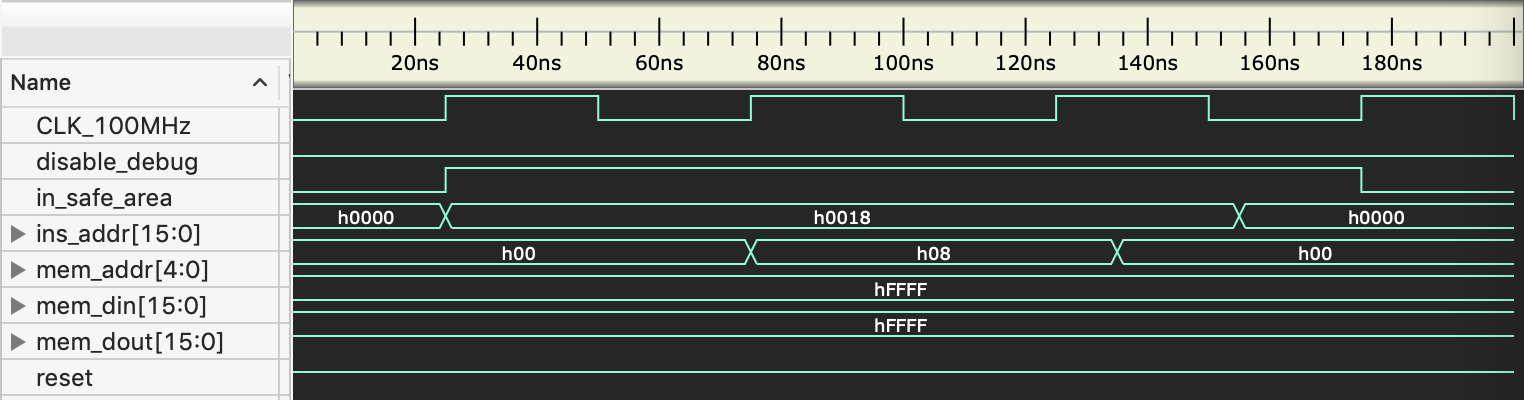
\includegraphics[width=1\textwidth]{figuras/ana1}
	\caption{Simulation of success access to the protected memory region.}
	\label{fig:ana1}
\end{figure}

Figure \ref{fig:ana1} shows a simulation that reflects the following steps: the instruction address go to  LOW\_CODE value; memory address go to a value inside protected region memory, in this case, LOW\_SAFE value; memory address go to 0x00; instruction address go to 0x0000. The module work as expected. In the first step, it correctly changes the \verb|in_safe_area| value to high, because it runs the first instruction of the safe code. As there was no memory access violation, no reset signal is triggered. 

\begin{figure}[h]
\centering
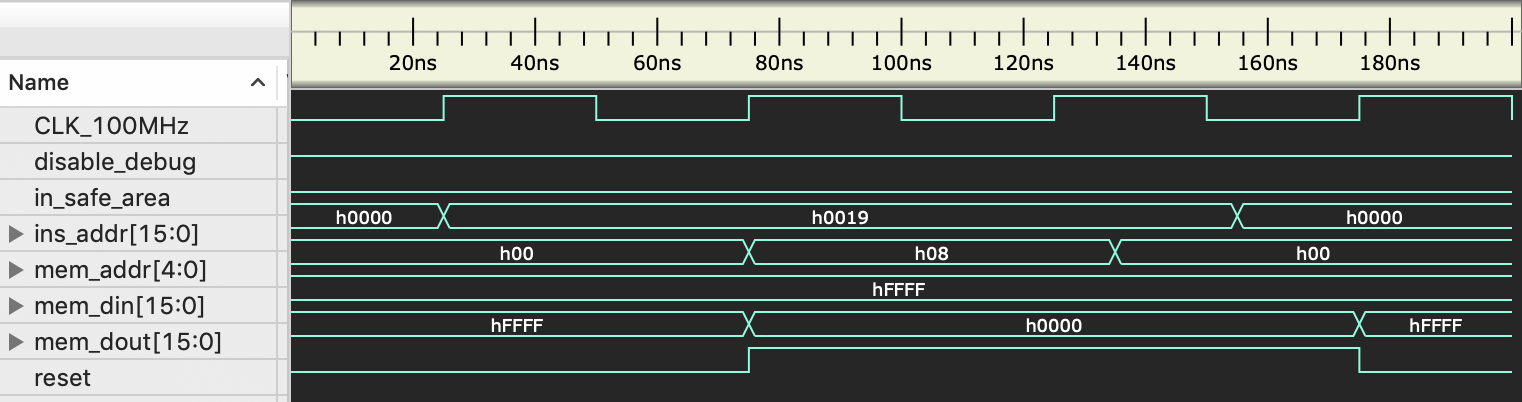
\includegraphics[width=1\textwidth]{figuras/ana2}
\caption{Simulation of what happens when the instruction pointer goes to the second code address and access to the protected memory region.}
\label{fig:ana2}
\end{figure}

The only difference from figure figure \ref{fig:ana1} and figure \ref{fig:ana2} is that in the first step  the instruction address go to  LOW\_CODE+1. Since this value is not the first instruction in safe code area, \verb|in_safe_area| stay with a low signal. In the second step, when there is an attempt to read a protected memory region, a reset signal is triggered. Another important aspect of this simulation is that the \verb|mem_din| pin is a constant value, but \verb|mem_dout| change to 0x0000 when the violation occurs. 

\begin{figure}[h]
	\centering
	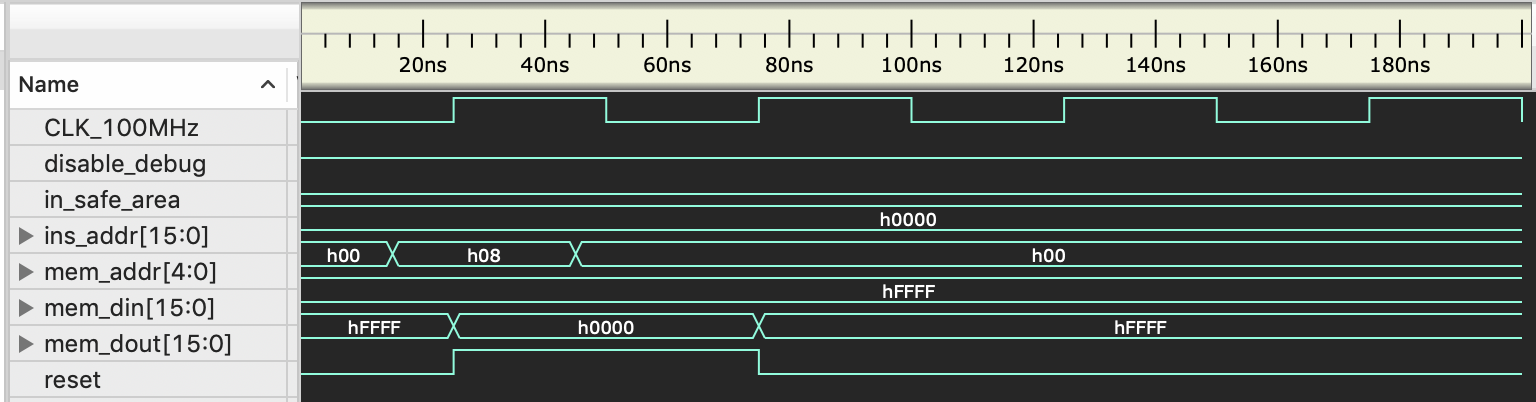
\includegraphics[width=1\textwidth]{figuras/ana3}
	\caption{Simulation of one not authorized access to the protected memory region.}
	\label{fig:ana3}
\end{figure}

Figure \ref{fig:ana3} is very similar to previous simulation. It shows a memory access violation.

\begin{figure}[h]
	\centering
	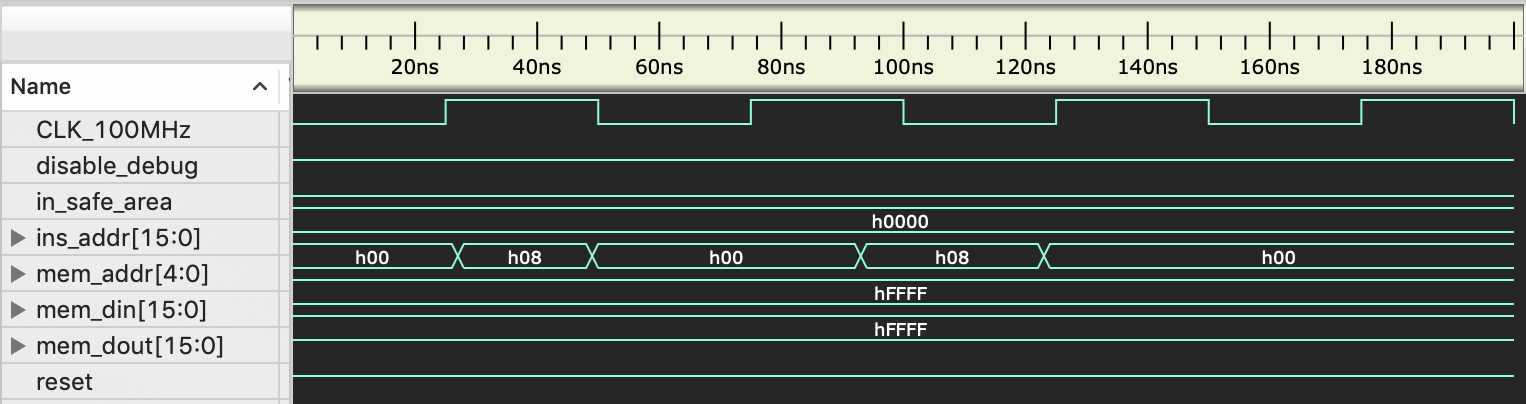
\includegraphics[width=1\textwidth]{figuras/ana4}
	\caption{Simulation of the behaviour when men\_addr pin inconsistency states happens.}
	\label{fig:ana4}
\end{figure}

The figure \ref{fig:ana3} aims to show that inconsistent states do not provoke accidental resets. In the image occur two inconsistent states, the first one is the change of \verb|mem_addr| between a half clock cycle (start at 22ns and ends at 48ns). The second one happens in the same pin, and start ate 93 ns and ended at 123ns.  

All images from the tests are generated using the Scansion\footnote{\url{http://www.logicpoet.com/scansion/}} application and the Icarus Verilog vvp runtime engine.

% parans are not showed in this table
